\documentclass[review]{elsarticle}

\usepackage{lineno,hyperref}
\modulolinenumbers[5]


% Packages rajoutés par PM
\usepackage{graphicx}
\usepackage{tikz}
\usetikzlibrary[positioning,arrows, arrows.meta]

% Packages rajoutés par NM
\usepackage[utf8]{inputenc} 
\usepackage{adjustbox}
\def\checkmark{\tikz\fill[scale=0.4](0,.35) -- (.25,0) -- (1,.7) -- (.25,.2) -- cycle;}
\def\lightcheckmark{\tikz\fill[scale=0.4](0,.35) -- (.25,0) -- (1,.7) -- (.25,.05) -- cycle;}

\journal{Journal of \LaTeX\ Templates}

%%%%%%%%%%%%%%%%%%%%%%%
%% Elsevier bibliography styles
%%%%%%%%%%%%%%%%%%%%%%%
%% To change the style, put a % in front of the second line of the current style and
%% remove the % from the second line of the style you would like to use.
%%%%%%%%%%%%%%%%%%%%%%%

%% Numbered
%\bibliographystyle{model1-num-names}

%% Numbered without titles
%\bibliographystyle{model1a-num-names}

%% Harvard
%\bibliographystyle{model2-names.bst}\biboptions{authoryear}

%% Vancouver numbered
%\usepackage{numcompress}\bibliographystyle{model3-num-names}

%% Vancouver name/year
%\usepackage{numcompress}\bibliographystyle{model4-names}\biboptions{authoryear}

%% APA style
%\bibliographystyle{model5-names}\biboptions{authoryear}

%% AMA style
%\usepackage{numcompress}\bibliographystyle{model6-num-names}

%% `Elsevier LaTeX' style
%\bibliographystyle{elsarticle-num}
\bibliographystyle{elsarticle-num-names}
%%%%%%%%%%%%%%%%%%%%%%%

\begin{document}

\begin{frontmatter}

\title{Un apport de l’IA aux crises épidémiologiques \\ Kiss the Covid}



\author[cristal]{P.~Mathieu\corref{cor1}\fnref{fn1}}
\ead{philippe.mathieu@univ-lille.fr}

\cortext[cor1]{Corresponding author}
\fntext[fn1]{}

\author[cristal]{N.~Mauhé}
\ead{nicolas.mauhe@univ-lille.fr}

\address[cristal]{Univ. Lille, CNRS, Centrale Lille, UMR 9189 --  CRIStAL Lab, F-59000 Lille, France}


\begin{abstract}
  Lors d'une crise sanitaire liée à l'apparition d'une maladie
  infectieuse, il est impératif d'avoir des systèmes d'aide à la
  décision des politiques publiques (évolution de la maladie, immunité
  collective, nombres dates et durées de périodes de
  confinement). \\
  L'évolution d'une maladie infectieuse peut-être modélisée de
  différentes façons (approche centrée-individus, réseaux sociaux,
  équations mathématiques, modèles de flux).\\
  Toutes ces modélisations nécessite l'usage de paramètres pour
  calibrer le modèle.\\
  Plus il y a de paramètres, plus il est facile de coller aux
  données (tout comme il existe toujours un polynôme de degré $n$ qui passe par $n$ points).\\
  Certains modélisateurs pensent que plus les paramètres sont précis
  (et nombreux), plus le modèle sera fiable. C'est un course
  sans fin.\\
  L'important est de trouver l'essence du problème, le modèle le plus
  économe en paramètres (parcimonieux) rendant compte des
  phénomènes observés. \\
  L'IA est d'une grande aide pour éviter les biais et régler au mieux
  ces modèles.
\end{abstract}

\begin{keyword}
Infectious disease \sep SIR modelling \sep Decision support system \sep artificial intelligence
\MSC[2010] 00-01\sep  99-00
%http://www.ams.org/msc/msc2010.html
\end{keyword}

\end{frontmatter}

\linenumbers

\section{Introduction (ce qui se fait en épidémiologie)}

Depuis exactement un siècle et le papier séminal de Kermack et
McKendrick, la modélisation épidémiologique a pris une part
prépondérante dans l’étude de ces phénomènes complexes. La crise du
H1N1 en 2008 a nettement amplifié ce phénomène, faisant apparaître un
nombre important de modèle tous plus complexe les uns que les
autres. Dans ce papiers nous montrons que les techniques
d’intelligence artificielle Utilisées à bon escient, Permettent d’une
part de concevoir des modèles plus facile à comprendre et à utiliser
par les thématiciens et d’autre part de faciliter grandement la
conception d’outils d’aide à la décision pour les politiques
sanitaires.


Le modèle présenté s'appuie sur des taux de contagion
adaptable chaque jour, dont la valeur est automatiquement calculée par
apprentissage génétique.



Le modèle SIR de Kermack et McKendrick \cite{} a été proposé en 1927 pour expliquer la hausse et la baisse rapides du nombre de patients infectés observées lors d’épidémies telles que la peste (à Londres en 1665, à Bombay en 1906) ou le choléra (à Londres en 1865). Il a été remis à l’avant-plan à la fin des années 1970 par Anderson et May \cite{}.


\bigskip


\hfill \scalebox{.75}{
	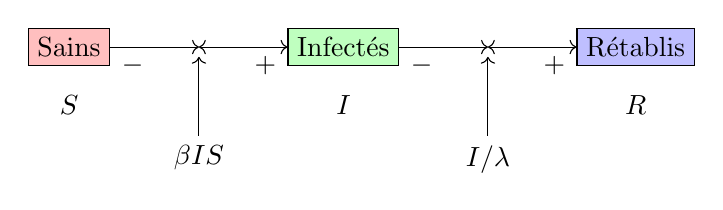
\begin{tikzpicture}[node distance=1cm,
          boite/.style={draw,rectangle, minimum width=1cm, fill=#1!25}]
          \node[boite=red](leftNode) {Sains};
	        \node[below=0.25cm of leftNode](labelLeftNode) {\(S\)};
		\node[right=of leftNode](middleLeft) {};
		\node[boite=green,right=of middleLeft](centralNode) {Infectés};
		\node[below=0.25cm of centralNode](labelCentralNode) {\(I\)};
		\node[right=of centralNode](middleRight) {};
		\node[boite=blue,right=of middleRight](rightNode) {Rétablis};
		\node[below=0.25cm of rightNode](labelRightNode) {\(R\)};
		\draw[->] (leftNode) --node[below, near start]{\(-\)} (middleLeft.center);
		\draw[<->] (middleLeft.center) --node[below, near end]{\(+\)} (centralNode);
		\draw[->] (centralNode) --node[below, near start]{\(-\)} (middleRight.center);
		\draw[<->] (middleRight.center) --node[below, near end]{\(+\)} (rightNode);
		\node[below=of middleLeft](leftLabel){\(\beta I S\)};
		\node[below=of middleRight](rightLabel){\(I / \lambda\)};
		\draw[->] (leftLabel) -- (middleLeft);
		\draw[->] (rightLabel) -- (middleRight);
	\end{tikzpicture}
} \hfill \


\begin{table}
\begin{adjustbox}{center}
\resizebox{18cm}{!}{%
\begin{tabular}{p{4cm}|p{4cm}|p{2cm}|p{2cm}|p{4cm}|p{11cm}}
  Article & Type & Statut & Zone & Paramètres & Objectif\\
  \hline

  \citet{benvenuto_application_2020} (ARIMA) & Statistical & Published & China & ... & Prediction de l'incidence et de la prévalence\\
  \citet{zlojutro_decision-support_2019} & Stochastic metapopulation epidemic model & Published & World & X cities, 4 compartments each & Number of cases and cities at risk  \\
  \citet{chinazzi_effect_2020} (GLEAM) & Stochastic metapopulation epidemic model & China & Published & 3200 subpopulations, 4 compartments each & Impact of travel restriction  \\
  \citet{scire_reproductive_2020} & Poisson process & Published & Switzerland & ... & Estimation of the reproductive number R  \\
  \citet{li_substantial_2020} & Stochastic metapopulation epidemic model & Published & China & 375 cities, 5 compartments each & Estimation of the prevalence and contagiousness \\

  \citet{flaxman_report_2020} & Statistical & Preprint & Europe & / & R0, Part de contaminés, Impact du confinement, Prévisions des décès \\
  \citet{ferguson_report_2020} & Agent-based & Preprint & Great Britain & 58 millions agents\footnote{REF 5 du papier} & Prediction of ICU and deaths according to lockdown scenarios  \\
  \citet{di_domenico_expected_2020} & Compartmental epidemic model & Preprint & Paris region & 11 compartments, 3 age classes & Estimation of propagation, Prediction of ICU, Deaths according to scenarios \\
  \citet{wilder_role_2020} & Agent-based model & Preprint & Hubei, Lombardy & 10 millions agents & Impact of age distribution and familial
household contacts on transmission  \\
  \citet{simha_simple_2020} & Compartment model & Preprint & Inde & 3 compartments & Prediction of cases, Lockdowns impact  \\
  \citet{roux_covid-19_2020} & Compartmental model & Preprint & France & 8 compartments x 17 age groups & Impact of lockdown on cases, deaths\\
  \citet{salje_estimating_2020} & ... & Preprint & France & 6 compartments x 8 age x 2 sex groups &Estimation du R0, et de la part de la pop infectée / décédée, impact du lockdown sur R0.  \\
  \citet{team_forecasting_2020} & Statistical & Preprint & Europe \& USA & ... & Prediction of deaths and hospital demand \\
  \citet{luo_predictive_2020} & Compartmental model & Preprint & Singapour, USA, Italie, Bresil & 3 compartimments & Prediction du nombre de cas  \\
  \citet{branas_flattening_2020} & Metapopulation epidemic model & Preprint & USA & 3108 Counties, 5 compartments each & Prediction of hospital and ICU beds, and deaths  \\
  \citet{keskinocak_impact_2020} &  Agent-based & Preprint & Georgia (USA) & 1 million agents & Impact of Social Distancing sur décès et infections  \\
  \citet{wang_spatiotemporal_2020} (STEM) & Compartmental model & Preprint & USA & 3 compartments x 3,104 counties & Prediction of deaths and cases \\
  \citet{li_overview_2020} (DELPHI) & Compartmental model & Documentation & World & 11 compartments & Impact mesures, prédiction nombre de cas et nombre de morts  \\
  \citet{woody_projections_2020} & Statistical & Preprint & USA & 50 states & Predict the number of deaths  \\
  \citet{platen_stochastic_2020} & Compartment model & Preprint & Australia & 4 compartments & Propagation number, Predicted number of deaths and cases  \\
  \citet{arenas_mathematical_2020} & Metapopulation epidemic model & Preprint & Spain & 19 regions, 7 compartments each & Prediction of number of cases  \\
  \citet{sanche_high_2020} & Poisson model \& Compartmental model & Preprint & Wuhan & 7 compartments & Estimate epidemiological parameters (R0, incubation period, etc.)  \\
  \citet{aleta_modeling_2020} & Agent-based & Preprint & Boston & 85k agents & Impact of distancing measures  \\
  REF TUOMISTO & Agent-based & Preprint & Helsinki & ... & Impact of simulated 	mobility restriction on hospitalized, ICU and Deaths \\

\end{tabular}}
\end{adjustbox}
\caption{Description des modèles épidémiologiques proposés durant l'épidémie de COVID-19}
\label{table:1}
\end{table}


Poisson process : ref ferguson.


\section{L'apport de l'informatique}

L'usage de l'IA est une méthode nouvelle pour l'épidémiologie, mais ancienne pour l'informatique.


Certains pensent que si on complexifie le modèle, on s'approche de la réalité : or plus il y a de paramètres, plus c'est facile de ``fitter'' : Problématique de l'overfitting (mettre une belle courbe qui passe par n points alors qu'en fait c'est une droite qui généralise le mieux).


\begin{figure}[h]
  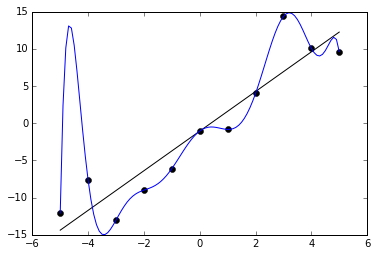
\includegraphics[width=0.8\linewidth]{Overfitted_Data.png}  
  \centering
  \caption{\copyright \href{wikipedia}{https://en.wikipedia.org/wiki/Overfitting}  Des données bruitées (approximativement linéaires) sont approximées par une fonction linéaire et une fonction polynomiale. Bien que la fonction polynomiale soit parfaitement ajustée, on constate que la fonction linéaire généralise surement bien mieux}
  \label{fig:overfitting}
\end{figure}


Un modèle qui ne fonctionne pas (parce que par exemple des R0 sont délirants) peut très bien néanmoins ``fitter'' les données  et donc continuer à prédire correctement les personnes en Réa


L'apport de l'informatique :
\begin{itemize}
\item des techniques et des outils : algos d'apprentissage
\item s'attacher à l'essence du problème : principe de parcimonie
\end{itemize}

\section{Cinq principes issus de l'informatique}

\textit{(Ici on peut décomposer en 1) définition du problème en épidémiologie puis 2) solutions apportées par l'informatique)}

\subsection{Nécessité}

Les modèles d'épidémie vont du simple modèle SIR que l'on peut résoudre sur un coin de feuille à des modèles réunissant des centaines d"agents indépendants, placés sur des cartes reproduisant des pays entiers (REF nécessaire). Les progrès informatiques rendent possible toutes les constructions auxquelles les épidémiologistes peuvent penser. Quel doit être le principe qui guide les choix des modélisateurs ? 

Un principe central dans la littérature informatique est celui de \textit{nécessité}. Chaque élément d'un modèle doit être nécessaire, et cette nécessité doit être justifiée.

A détailler : interaction avec validation. 
1) Rapport complexité / fitting
2) Rapport justification / validation  (si non validé, alors doit être justifié)

\subsection{Calibration}

Tout modèle qui vise à estimer un élément de la réalité non accessible (comme le taux de propagation) ou à prédire un élément empirique doit être calibré sur des éléments réels. Si ce principe n'est pas respecté, il est possible de produire un modèle qui semble tout à fait répondre aux objectifs fixés mais qui décrit en fait un tout autre phénomène. (Illustration modèle python).

Il s'agit d'un aspect central dans modélisation informatique et l'apprentissage informatique. Les principes de calibration issus de cette littérature peuvent être adaptés aux modèles épidémiologiques.

\subsection{Approximation}

Les possibilités induites par la modélisation donnent souvent l'illusion de la précision. On lit par exemple dans la presse des estimations très précises après la virgule produites par des modèles épidémiologiques portant sur des éléments très difficiles à estimer : c'est le cas par exemple des estimations du nombre d'infectés ou dut aux de propagation, souvent rapportées avec trois chiffres après la virgule (REF 4,4\% presse). 

Ces analyses ignorent une question déterminante : le phénomène est-il capturable entièrement par des moyens computationnels ? Parfois le mécanisme à l'oeuvre est une dynamique changeante dont la prévision est hors de notre portée : c'est le cas des mutations possibles du COVID-19 au cours de l'épidémie, ou de sa réaction face à l'environnement. C'est particulièrement vrai lorsque l'on s'attaque à des dynamiques sociales, déterminantes dans le calcul du taux de propagation. La difficulté de modéliser les comportements humains et leur agrégation au niveau de la société est un challenge considérable, qui nourrit une littérature particulièrement active parmi les discipline informatiques. Il est possible de tirer de nombreux enseignements de cette littérature à destination de l'épidémiologie : le principal est sans doute le recul nécessaire relatif à la précision des estimations et des prévisions des modèles impliquant des décisions humaines (REF article JASSS).

Un autre aspect relativement méconnu du grand public relatif aux modèles épidémiologiques est la sensibilité aux paramètres initiaux. Un changement relativement faible des conditions initiales peut conduire à des modélisations très différentes. Il s'agit d'un aspect bien connu des disciplines informatiques, étudié notamment par les sciences de la complexité. 

***

Le problème vient du fait que l'approximation n'est pas une fonction "native" des nouveaux outils proposés à l'épidémiologie. La simulation informatique d'un modèle tel que les modèles par agents ou les modèles compartimentaux nécessitent des input fixes et donnent des résultats tout aussi fixes : une prédiction telle que "2452 décès" constituera alors un résultat. C'est donc une étape supplémentaire que d’insuffler l'approximation à ces modèles là. Soit en transmettant la véritable approximation des entrées, en réalisant plusieurs scénarios avec des valeurs différentes. Soit mathématiquement, en transformant une entrée en distribution de probabilité ce qui permet d'obtenir un résultat aléatoire, que l'on pourra alors caractériser à l'aide d'intervalles de confiance. Soit, si l'approximation provient de mécanismes stochastiques à l'intérieur du modèle, en procédant à un grand nombre de simulations qui permettront d'estimer le caractère aléatoire du résultat, par exemple via une moyenne et un écart-type du nombre de décès prédits. Dans de nombreux cas, la modélisation réclamera une combinaison de ces éléments là.

\subsection{Validation}

L'épidémie de COVID-19 peut être modélisée de manière très différente, même si l'on s'accordait sur les caractéristiques de base du virus. La question déterminante est donc de savoir si une modélisation est fidèle à la réalité qu'elle prétend simuler, voire prévoir. Il s'agit d'une problématique centrale en modélisation informatique, celle de la \textit{validation}.

La littérature informatique peut nous aider à nous prémunir contre un certain nombre d'écueils, comme celui de l'\textit{overfitting}. (...)

Pour aider à valider un modèle épidémiologique, plusieurs outils issus de la littérature informatique sont disponibles. Un exemple est celui de la \textit{cross-validation}. (...)

Attention : manipulation graphique (aplatissement : ROUX, colonnes : Luo)

Validation : 2 modèles : 

1) avec points au hasard
2) prédiction des derniers jours et comparaison avec la réalité (5 jours par exemple)


\subsection{Réplicabilité}



\section{Présence de ces principes dans les modèles actuels}

\begin{table}
\resizebox{\textwidth}{!}{%
\begin{tabular}{c|c|c|c|c|c}
  Article & Nécessité & Calibration & Approximation & Validation & Réplicabilité\\
  \hline

  \citet{benvenuto_application_2020} (ARIMA) &   & \checkmark &   &   & \checkmark  \\
  \citet{zlojutro_decision-support_2019} & \textasciitilde & \checkmark & \lightcheckmark & ... & \lightcheckmark \\
  \citet{chinazzi_effect_2020} (GLEAM) &   & \checkmark & \checkmark & ... & \lightcheckmark  \\
  \citet{scire_reproductive_2020} &   & \checkmark & \checkmark &   & \checkmark  \\
  \citet{li_substantial_2020} &   & \checkmark  & \checkmark  &   & \lightcheckmark \\

  \citet{flaxman_report_2020} & \checkmark & \checkmark & \checkmark & \checkmark & \checkmark \\
  \citet{ferguson_report_2020} &   & \checkmark &   &   &    \\
  \citet{di_domenico_expected_2020} & \lightcheckmark & \checkmark & \checkmark & \checkmark & \lightcheckmark \\ 
  \citet{wilder_role_2020} & \lightcheckmark & \checkmark & \checkmark & \checkmark & \checkmark  \\
  \citet{simha_simple_2020} & \lightcheckmark & \lightcheckmark & \checkmark & \lightcheckmark & \lightcheckmark \\
  \citet{roux_covid-19_2020} &   & \lightcheckmark & \lightcheckmark & \lightcheckmark &    \\
  \citet{salje_estimating_2020} &   & \lightcheckmark & \lightcheckmark & \lightcheckmark &    \\
  \citet{team_forecasting_2020} &   & \checkmark & \checkmark &   &    \\
  \citet{luo_predictive_2020} & \lightcheckmark & \checkmark & \checkmark &   &   \\
  \citet{branas_flattening_2020} &   & \checkmark & \checkmark &   &   \\
  \citet{keskinocak_impact_2020} &   & \checkmark &   & \lightcheckmark &    \\
  \citet{wang_spatiotemporal_2020} &   & \checkmark & \lightcheckmark & \lightcheckmark & \lightcheckmark \\
  \citet{li_overview_2020} & \lightcheckmark & \checkmark &   &   & \lightcheckmark \\
  \citet{woody_projections_2020} &   & \checkmark & \lightcheckmark & \checkmark &   \\
  \citet{platen_stochastic_2020} &   &   &   &   &    \\
  \citet{arenas_mathematical_2020} &   & \checkmark & \checkmark & \lightcheckmark & \lightcheckmark  \\
  \citet{sanche_high_2020} &   & \checkmark & \checkmark & \lightcheckmark &    \\
  \citet{aleta_modeling_2020} &   & \checkmark & \checkmark &   &    \\
  REF TUOMISTO & \lightcheckmark & \lightcheckmark &   & \lightcheckmark & \checkmark \\

\end{tabular}}
\caption{Présence des cinq principes dans les modèles épidémiologiques proposés durant l'épidémie de COVID-19}
\label{table:2}
\end{table}

Replicabilité : analyse du coût :
0 : Impossible
\lightcheckmark : Possible mais coût très élevé pour différentes raisons, avec plusieurs scénarios possibles:
- Tout est détaillé et clair mais pas de code
- Le code est disponible, tout est disponible, mais pas clair du tout et travail très important à mener

Checkmark : Réalisable, clair, expliqué, code disponible


[ANALYSE UNIQUEMENT POSITIVE]

Approximation :

Mentionner \cite{benvenuto_application_2020} : "The correlogram reporting the ACF and PACF showed that both prevalence and incidence of COVID- 2019 are not influenced by the seasonality."

\section{Un exemple simple}

\subsection{Fitting d'un modèle simple}

\begin{figure}
\begin{center}
  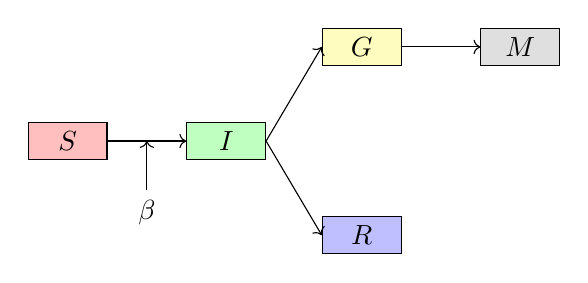
\begin{tikzpicture}[node distance=1cm,
    boite/.style={draw,rectangle, minimum width=1cm, fill=#1!25}]
    \node[boite=red](premier){\(S\)};
    \node[boite=green, right=of premier](second){\(I\)};
    \draw[->] (premier) -- node[midway](milieu){} (second);
    \node[below=.5cm of milieu](labelMilieu){\(\beta\)};
    \draw[->] (labelMilieu) -- (milieu.center);
    \node[boite=yellow, above right=of second](troisHaut){\(G\)};
    \draw[->] (second.east) -- (troisHaut.west);
    \node[boite=blue, below right=of second](troisBas){\(R\)};
    \draw[->] (second.east) -- (troisBas.west);
    \node[boite=gray, right=of troisHaut](quatre){\(M\)};
    \draw[->] (troisHaut) -- (quatre);
  \end{tikzpicture}
\end{center}
\caption{Le modèle épidémiologique par compartiments SIRGM}
\label{figure:SIRGM}
\end{figure}

Il s'agit d'un modèle SIRGM : une extension du modèle SIR aux deux catégories qui intéressent particulièrement les décideurs en ce qui concerne le COVID-19, à savoir le nombre de personnes en réanimation (R) et le nombre de décès (M). Incidemment, il s'agit des catégories pour lesquelles les données sont les plus fiables. Par opposition, le nombre d'infectés et le nombre d'hospitalisés souffrent d'un biais de sélection important et variable au cours du temps, dus à des changements de politiques publiques.

L'objet du modèle est de trouver les paramètres de ce modèle épidémiologique de sorte qu'il reproduise le plus fidèlement possible les données réelles. D'un point de vue informatique, il s'agit de fitter le plus précisément possible les courbes du nombre de lits occupés en réanimation et du nombre de décès. 

Certains paramètres du modèle épidémiologique ont fait l'objet d'études médicales : c'est le cas du temps de contagiosité et du taux de cas grave. Ils sont donc fixés à priori, et nous verrons à la section suivante les conséquences de les laisser libres.

un autre paramètre fixé à priori est celui du nombre d'infecté initial. D'après les données, 3 personnes ont été officiellement dépistées au début de la période, néanmoins le nombre d'infecté réel est probablement beaucoup plus élevé. Il n'y a pas de moyen de connaître précisément ce chiffre : nous l'avons fixé arbitrairement à 200. Ce paramètre interagit principalement avec le taux de propagation de la période initiale. Si le nombre d'infecté initial est moindre, le fitting de la courbe ajustera simplement le taux de propagation initial à la hausse et conservera les autres paramètres à un niveau très similaire. Il s'agit d'un avertissement supplémentaire relatif à une interprétation trop précise des taux de propagation : ils dépendent crucialement d'informations dont nous ne disposons pas.

La propagation du virus est le premier paramètre de ce type de modèle (c'est le bêta en Figure \ref{figure:SIRGM}, qui peut également être exprimé en termes de R0). Cependant, ce taux de propagation dépend du comportement humain, et donc des changements de politiques publiques en termes de confinement, de règles de distanciation sociale, etc. AU lieu de fixer un seul taux de propagation, nous en fixons donc quatre, soit un pour chaque grande période en France : la période initiale, une période d'une dizaine de jours précédant l'entrée en vigueur réglementaire du confinement strict, le confinement lui même, puis le dé-confinement. La période précédant le confinement a été marquée par des déplacements très importants de la population qui pouvait choisir son lieu de confinement, ce qui explique la nécessité de la prendre en compte.

Les autres paramètres sont les variables d'ajustement laissées libres pour obtenir un modèle épidémiologique cohérent avec les données observées.

Le problème devient dès lors un problème d'optimisation, et plusieurs techniques s'ouvrent à nous pour fitter le modèle. Nous avons utilisé un algorithme génétique basique. Les résultats sont reportés en Table \ref{table:meilleur} et en Figure \ref{figure:meilleur}.

\begin{table}
\small
\begin{center}
\begin{tabular}{|c|c|}
    \hline
R0 avant & 1.77\\ 
R0 pré-confinement & 3.47 \\ 
R0 confinement & 0.52\\ 
R0 déconfinement & 0.76\\ 
Infectés initiaux & 200.0\\ 
Taux réanimation & 0.005\\ 
Taux remis & 0.1\\ 
Taux réanimation vers grave & 0.025\\ 
Taux réanimation vers décès & 0.064\\ 
 
      \hline
\end{tabular}
\end{center}
\caption{Paramètres du modèle SIGRM.}
\label{table:meilleur}
\end{table}

\begin{figure}
\begin{center}
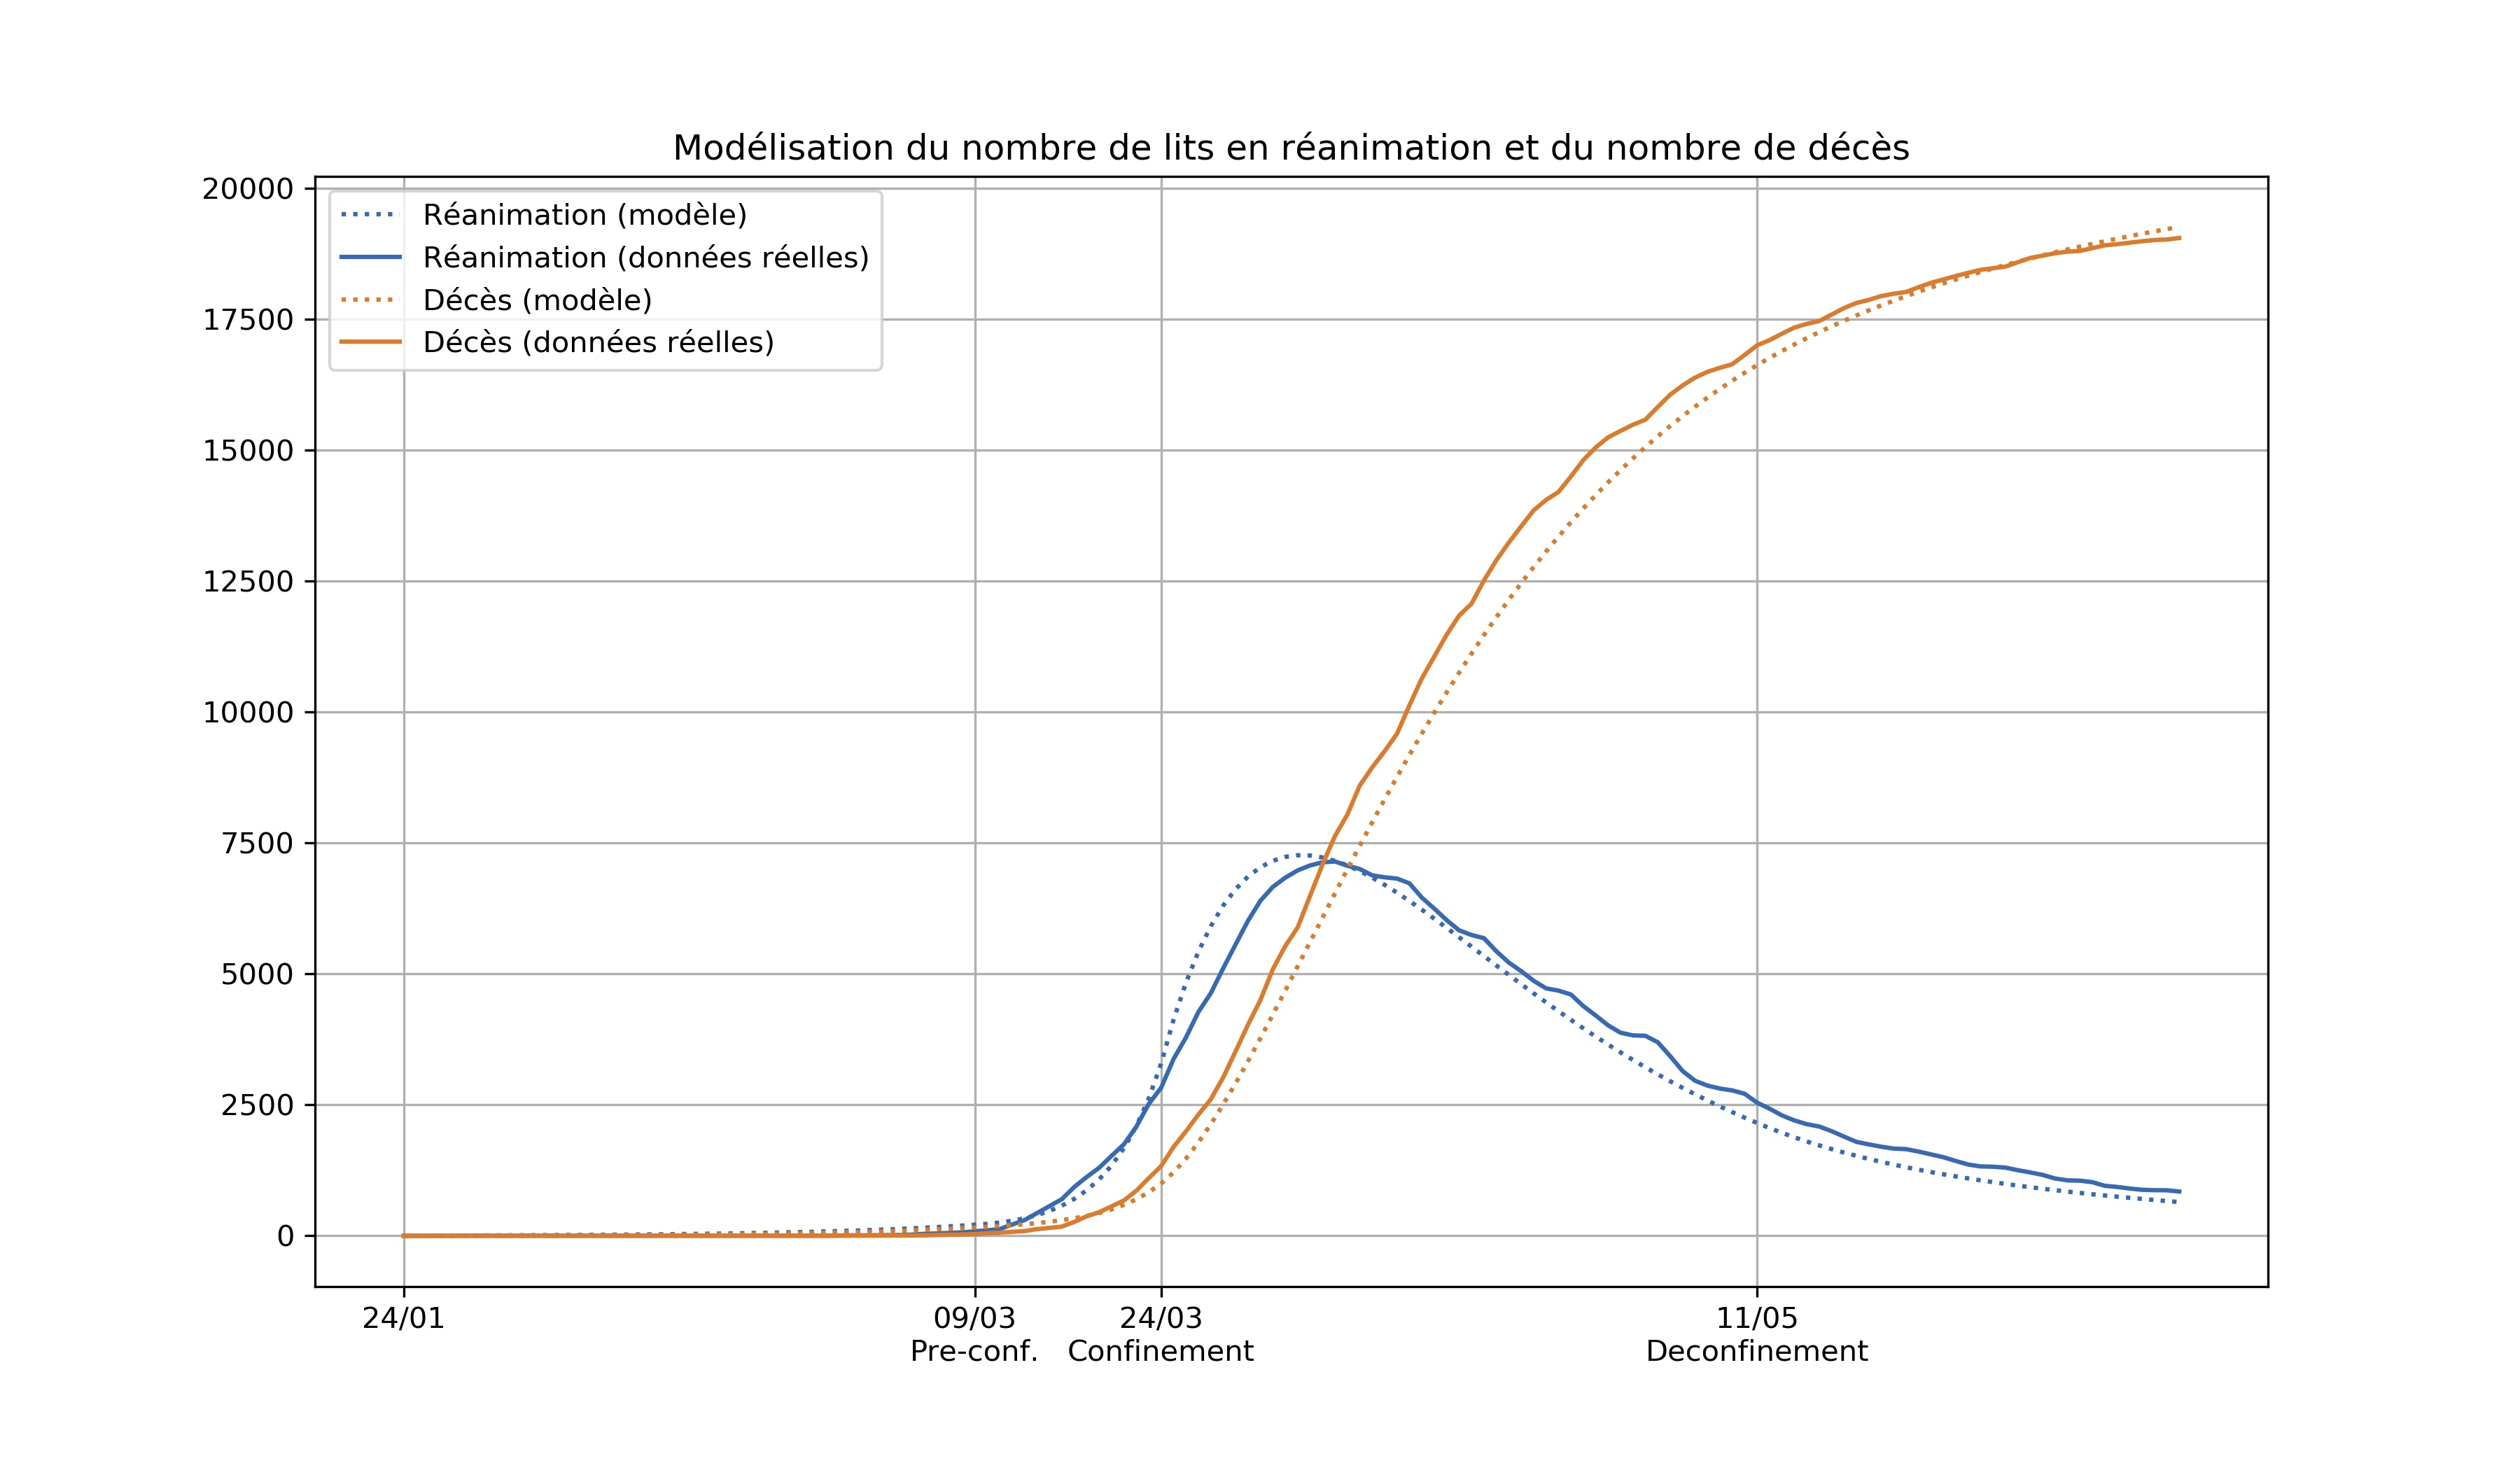
\includegraphics[width=1\linewidth]{figures/meilleur.jpg}
\end{center}
\caption{Le modèle SIGRM avec les paramètres donnés en Table \ref{table:meilleur} correspond aux données.}
\label{figure:meilleur}
\end{figure}

Le modèle fitte raisonnablement bien les données, et ce avec une structure très simple. Les paramètres estimés sont cohérent avec la littérature scientifique portant sur le COVID-19. 

\subsection{Progression des médecins}

Ce type de modèle peut néanmoins ignorer certains phénomènes qui viendraient changer les paramètres au cours du temps. C'est par exemple le cas des taux de mortalité, qui peuvent être affectés par la progression du corps médical sur le sujet. Des entretiens avec des responsables du CHU de Lille nous ont informé de l'amélioration du traitement des personnes en réanimation. Ce type de phénomène est compatible avec une modélisation légèrement différente de l'épidémie, comme en témoigne la Figure \ref{figure:medecins}.

\begin{table}
\small
\begin{center}
\begin{tabular}{|c|c|}
    \hline
R0 avant & 1.95\\ 
R0 pré-confinement & 2.76 \\ 
R0 confinement & 0.64\\ 
R0 déconfinement & 0.76\\ 
Infectés initiaux & 200.0\\ 
Taux réanimation & 0.005\\ 
Taux remis & 0.1\\ 
Taux réanimation vers grave & 0.025\\ 
Taux réanimation vers décès & 0.07\\ 
 
      \hline
\end{tabular}
\end{center}
\caption{Paramètres du modèle intégrant la progression du traitement.}
\label{table:medecins}
\end{table}

\begin{figure}
\begin{center}
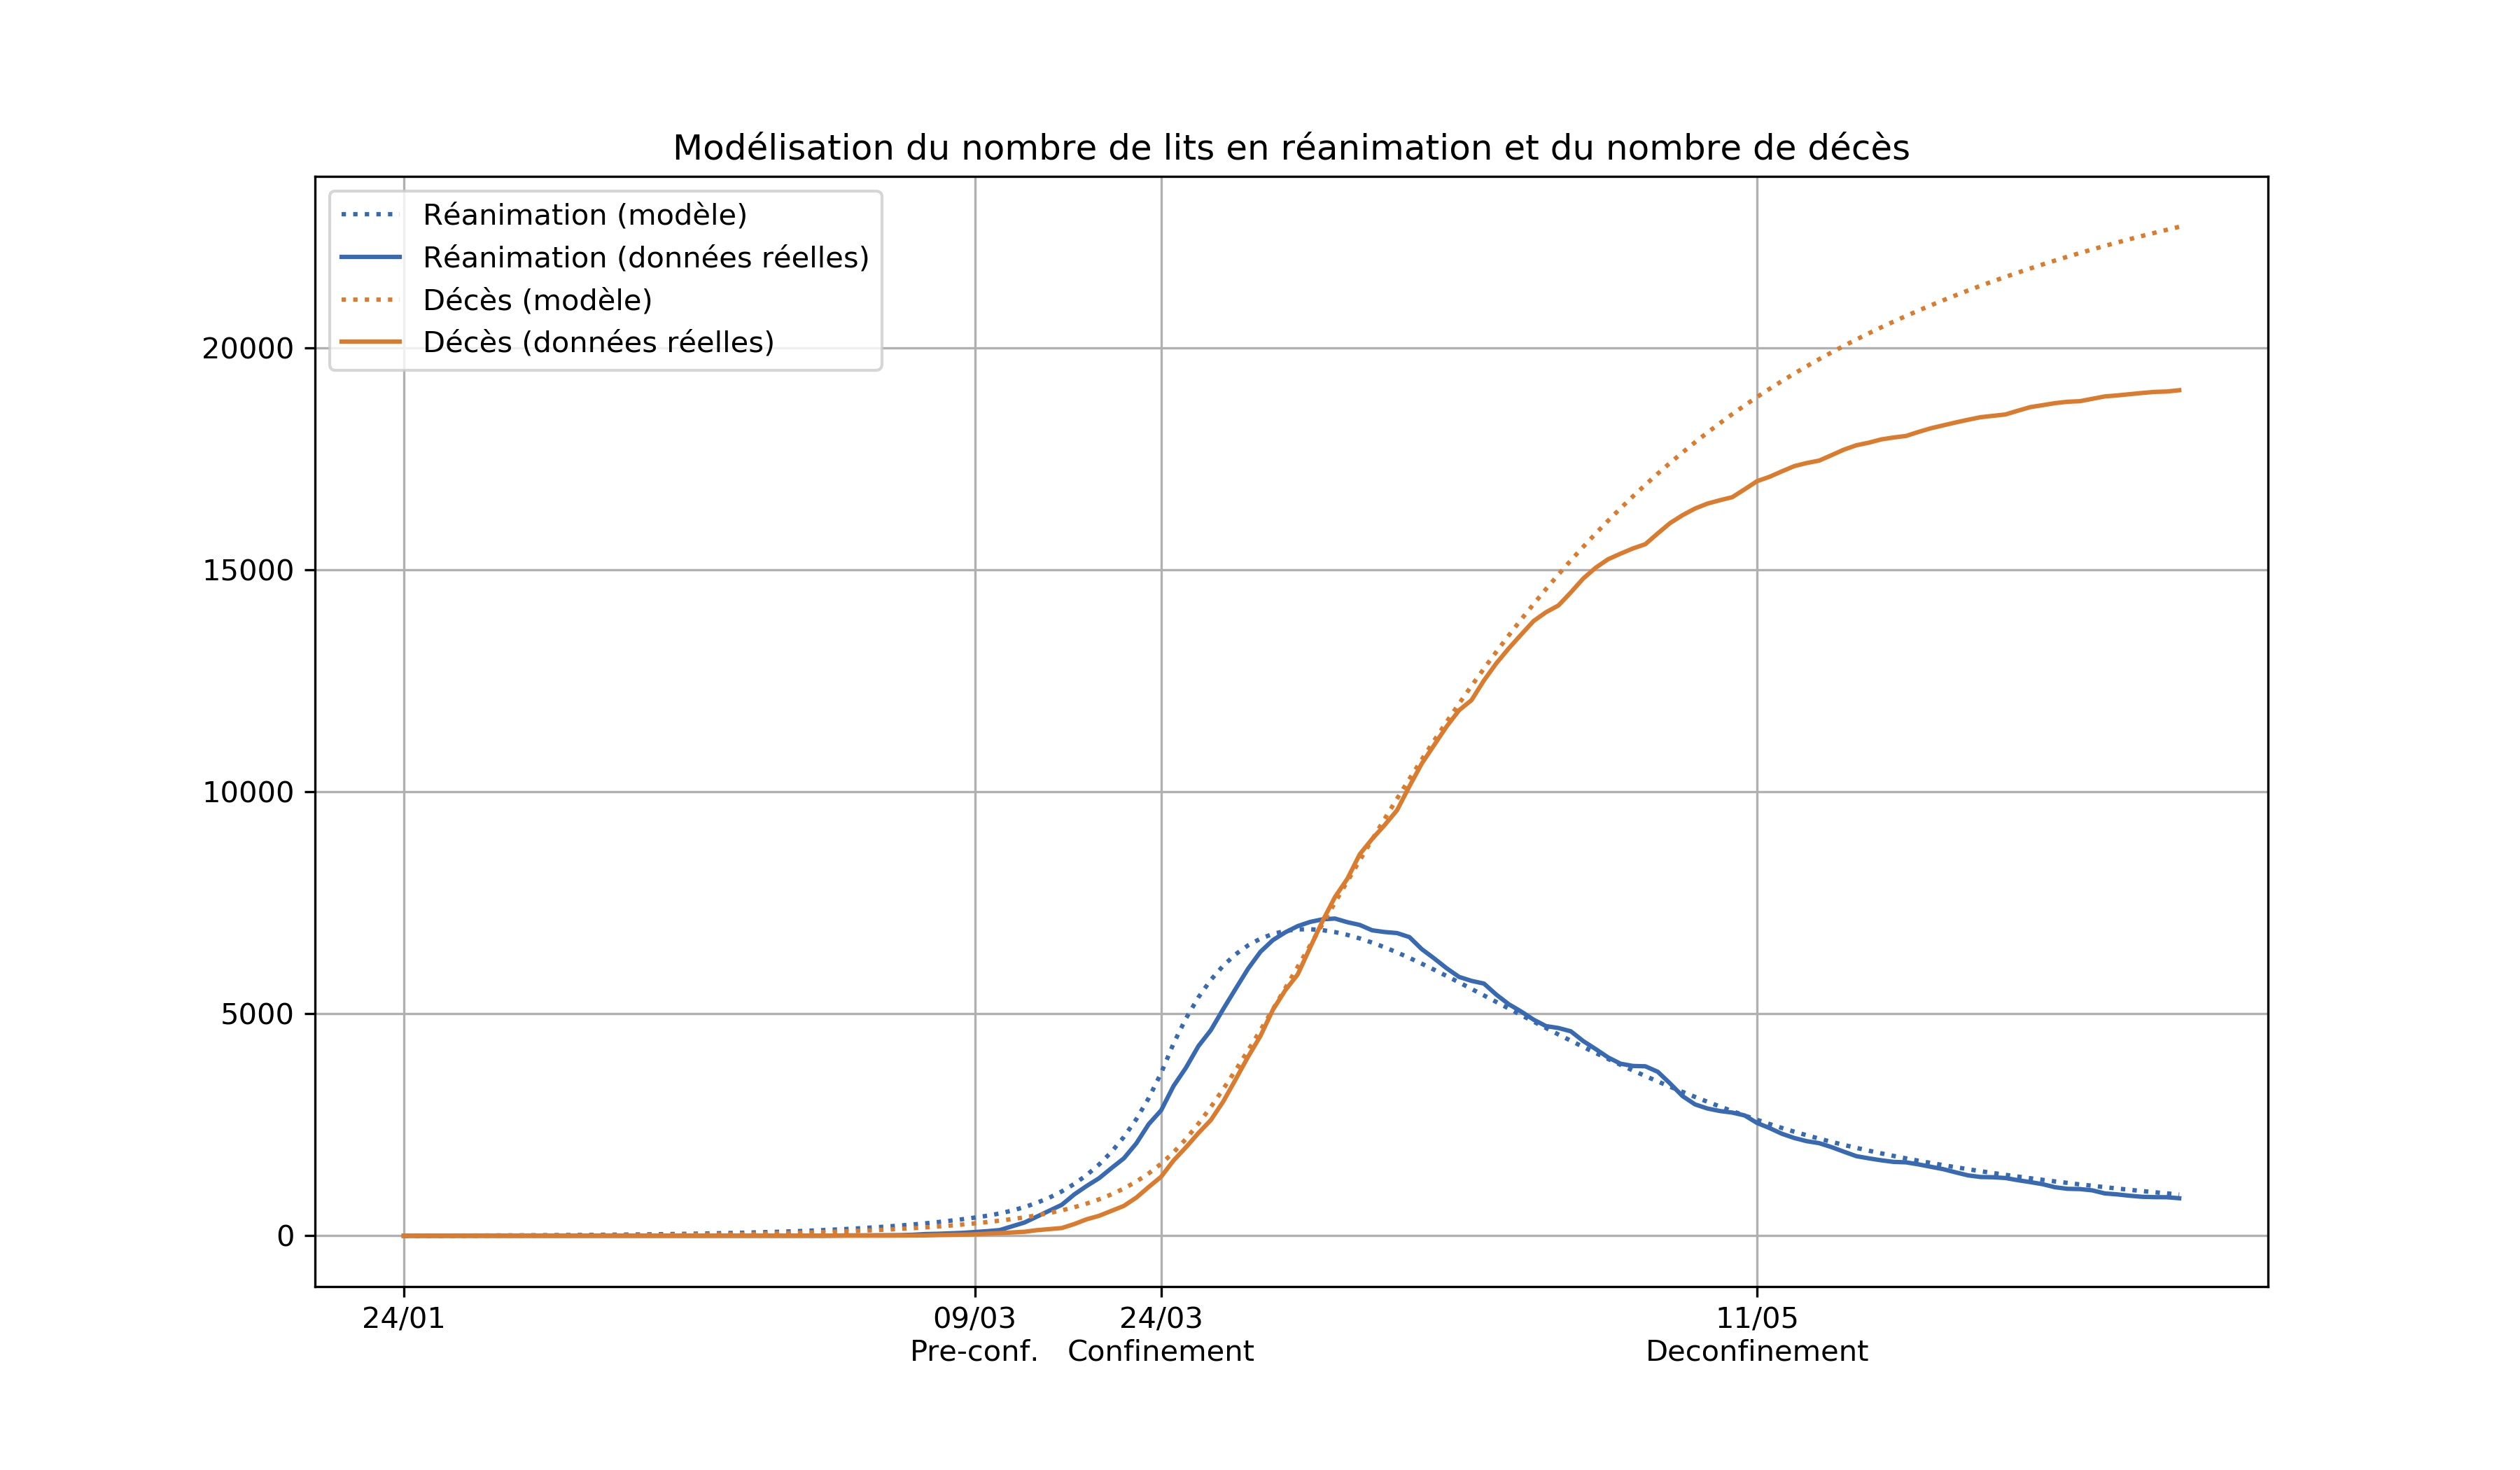
\includegraphics[width=1\linewidth]{figures/medecins.jpg}
\end{center}
\caption{Les donnnées réelles sont compatibles avec une modélisation épidémiologique intégrant la progression du traitement des patients en réanimation.}
\label{figure:medecins}
\end{figure}

On observe que le modèle permet un meilleur fitting des entrées en réanimation si la courbe des décès est autorisée à décrocher progressivement de celle prévue par le modèle. Cela témoigne du fait qu'intégrer la progression des médecins améliorerait le fitting des données. Il y a donc un arbitrage a réaliser en termes de perte de simplicité versus l'amélioration de la prédictabilité du modèle.

\subsection{Des paramètres laissés libres}

Le danger de laisser trop de paramètres libres pour l'optimisation est d'obtenir une modélisation plus performante mais qui correspond à un tout autre virus. Prenons l'exemple du temps de contagiosité : on sait désormais que c'est une des caractéristiques singulières du COVID-19, qui présente des temps d'incubation et de contagiosité très importants comparés aux autres virus.

Si l'on laisse le temps de contagiosité libre dans la modélisation (via le taux S vers I), on peut obtenir une modélisation telle que décrite dans la Table \ref{table:faux} et la Figure \ref{figure:faux}.

\begin{table}
\small
\begin{center}
\begin{tabular}{|c|c|}
    \hline
R0 avant & 1.2\\ 
R0 pré-confinement & 1.16 \\ 
R0 confinement & 1.14\\ 
R0 déconfinement & 1.34\\ 
Infectés initiaux & 200.0\\ 
Taux réanimation & 0.001\\ 
Taux remis & 0.781\\ 
Taux réanimation vers grave & 0.006\\ 
Taux réanimation vers décès & 0.062\\ 
 
      \hline
\end{tabular}
\end{center}
\caption{Paramètres clairement différents de l'épidémie de COVID-19}
\label{table:faux}
\end{table}

\begin{figure}
\begin{center}
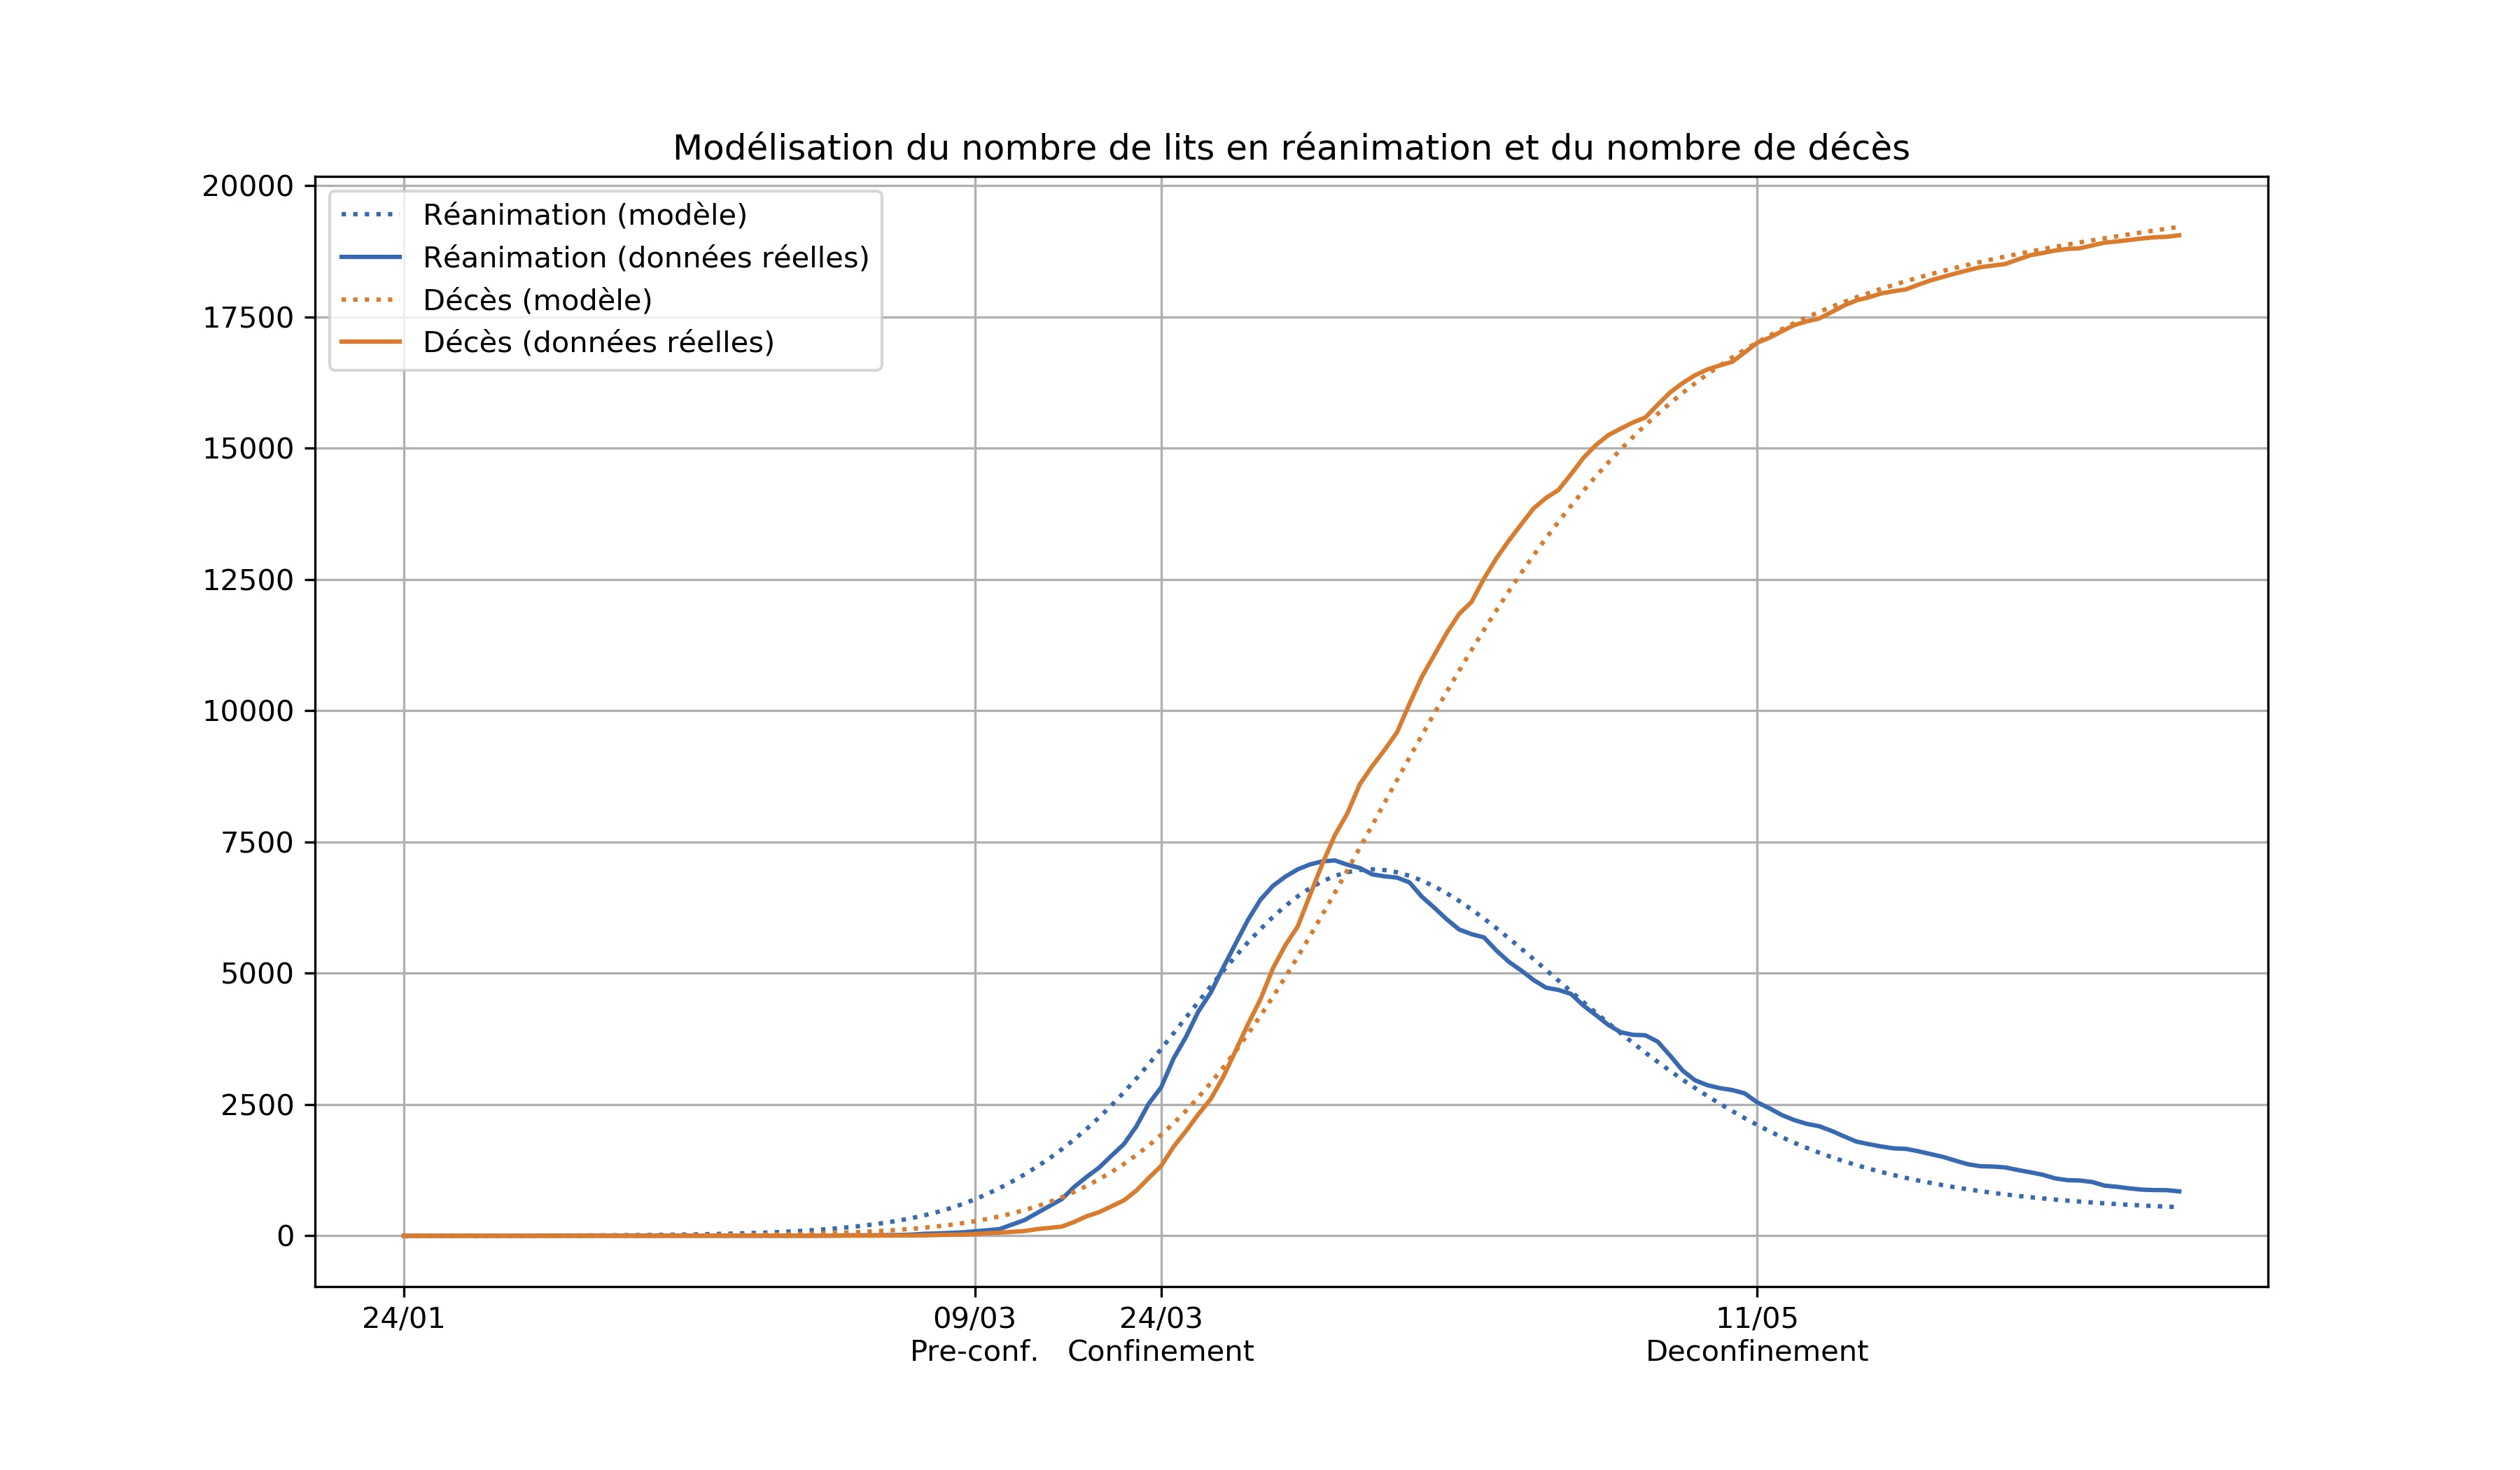
\includegraphics[width=1\linewidth]{figures/faux.jpg}
\end{center}
\caption{La modélisation issue des paramètres de la Table \ref{table:faux} donne de bons résultats.}
\label{figure:faux}
\end{figure}

Il s'agit de la modélisation d'un virus très faiblement mortel, qui présente un temps de contagiosité réduit (entre un et deux jours) et qui se serait répandu dans la population avec un R0 en permanence supérieur à 1. L'épidémie aurait atteint son pic et faiblirait désormais car le seuil de l'immunité collective serait atteint, et 88\% de la population aurait contracté ce virus.

Cette modélisation correspond aux données observées : en l'absence de spécification volontaire de données médicales observées par ailleurs, il est donc tout à fait possible d'obtenir un modèle épidémiologique très différent de l'épidémie réelle, mais qui présenterait les mêmes statistiques observables.

\section*{References}

\bibliography{kiss_covid}
\nocite{*}

\end{document}

\iffalse

\bigskip

\hfill \scalebox{.75}{
  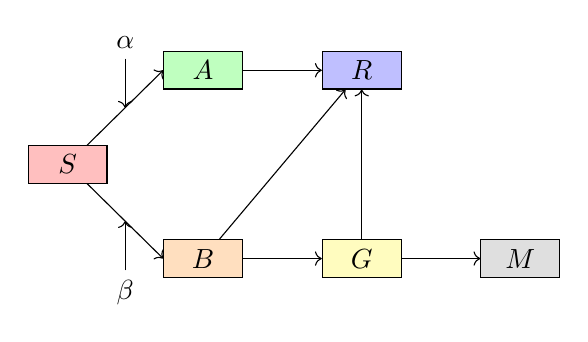
\begin{tikzpicture}[node distance=1cm,
    boite/.style={draw,rectangle, minimum width=1cm, fill=#1!25}]
    \node[boite=red](premier){\(S\)};
    \node[boite=green, above right=of premier](secondHaut){\(A\)};
    \draw[->] (premier) -- node[midway](milieuHaut){} (secondHaut.west);
    \node[above=.5cm of milieuHaut](labelMilieuHaut){\(\alpha\)};
    \draw[->] (labelMilieuHaut) -- (milieuHaut.center);
    \node[boite=orange, below right=of premier](secondBas){\(B\)};
    \draw[->] (premier) -- node[midway](milieuBas){} (secondBas.west);
    \node[below=.5cm of milieuBas](labelMilieuBas){\(\beta\)};
    \draw[->] (labelMilieuBas) -- (milieuBas.center);
    \node[boite=blue, right=of secondHaut](troisHaut){\(R\)};
    \draw[->] (secondHaut) -- (troisHaut);
    \draw[->] (secondBas) -- (troisHaut);
    \node[boite=yellow, right=of secondBas](troisBas){\(G\)};
    \draw[->] (secondBas) -- (troisBas);
    \draw[->] (troisBas) -- (troisHaut);
    \node[boite=gray, right=of troisBas](quatre){\(M\)};
    \draw[->] (troisBas) -- (quatre);
  \end{tikzpicture}
} \hfill \



\begin{center}
  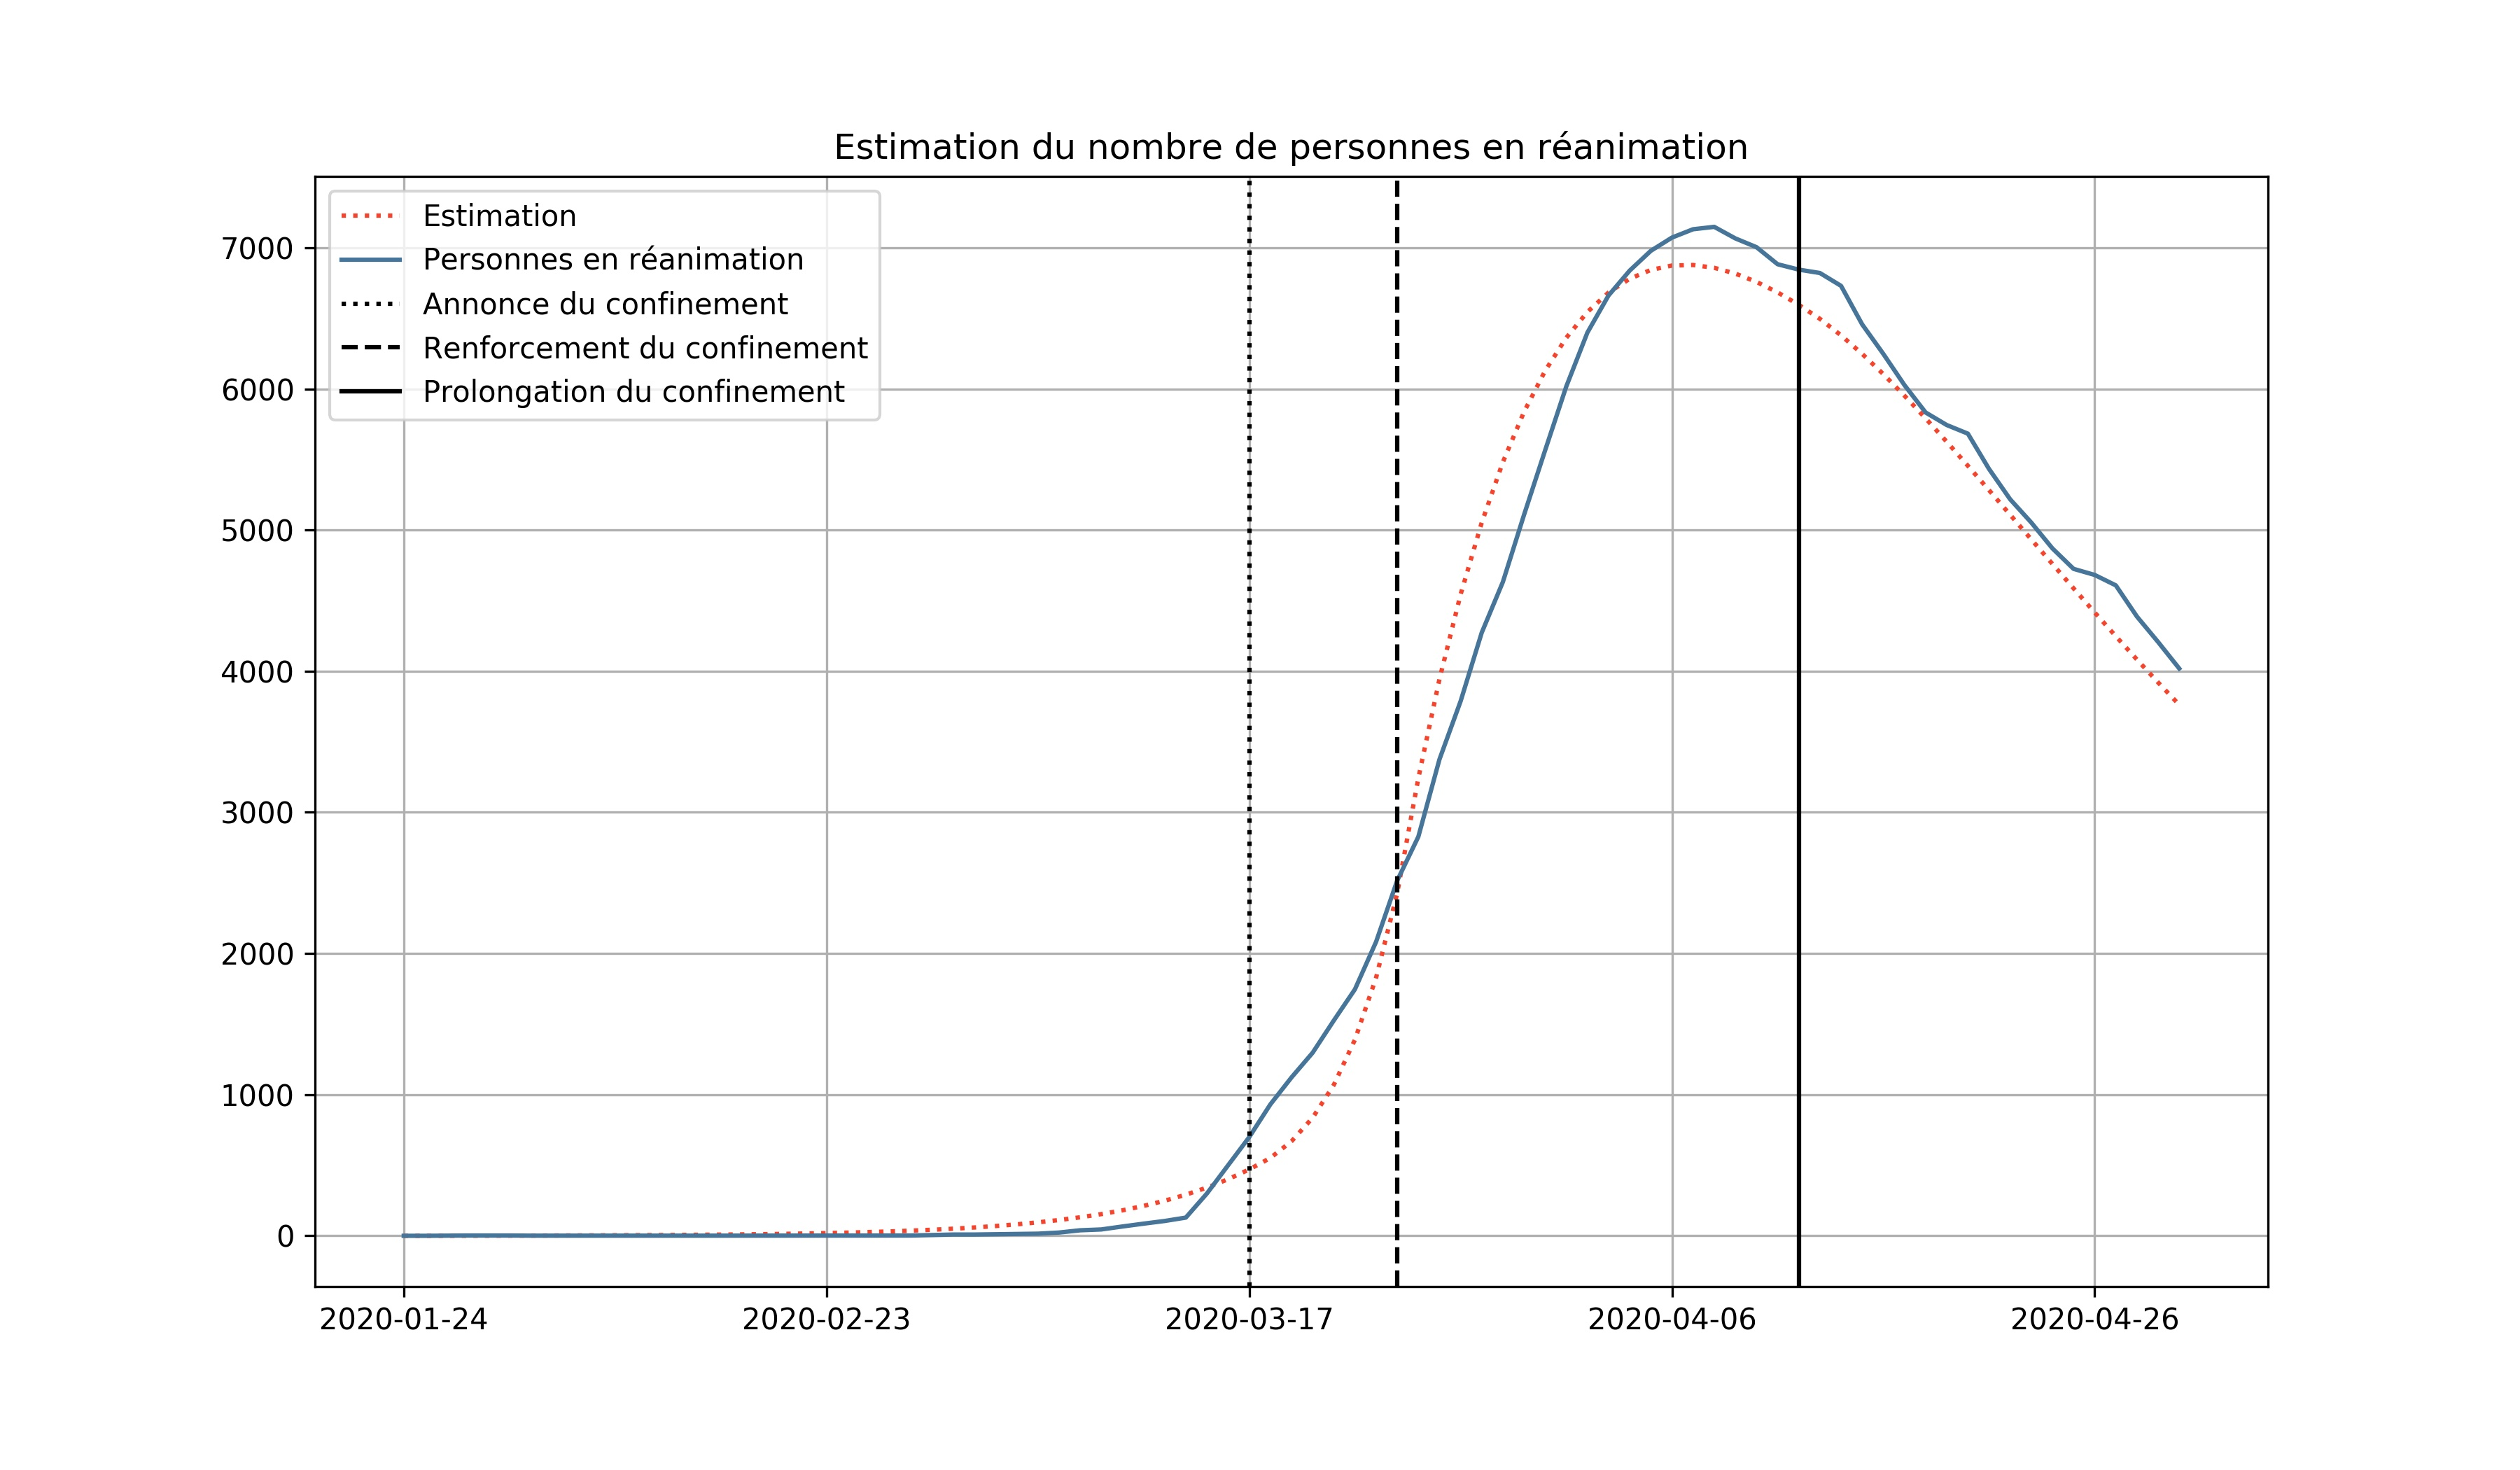
\includegraphics[width=0.8\linewidth]{../slides/figure1.jpg}
\end{center}

\fi
